\documentclass[11pt,a4paper]{article}

\usepackage[T1]{fontenc}
\usepackage[english]{babel}
\usepackage{lmodern,microtype}
\usepackage[a4paper,top=2.6cm,bottom=2.8cm,left=2.5cm,right=2.5cm]{geometry}
\usepackage{amsmath,amssymb,amsthm,mathtools}
\usepackage{xcolor}
\usepackage{tikz}
\usetikzlibrary{arrows.meta}
\usepackage[colorlinks=true,linkcolor=blue!65!black,citecolor=teal!70!black,urlcolor=blue!65!black,linktoc=all]{hyperref}
\hypersetup{
  pdftitle={Type II1 Operator-Algebra Quantum Error Correction for a de Sitter Causal Diamond: A Speculative Perspective on a Holographic Universe},
  pdfauthor={Murat Durmus}
}

\definecolor{diagramink}{HTML}{243745}
\definecolor{diagramborder}{HTML}{557489}
\definecolor{diagramfill}{HTML}{F2F6F8}
\definecolor{diagrambalance}{HTML}{FBF4E9}
\definecolor{diagramwarm}{HTML}{8C622C}

\tikzset{
  paper diagram/.style={font=\small,text=diagramink,>=Latex},
  paper box/.style={
    draw=diagramborder, fill=diagramfill, rounded corners=2pt,
    line width=.55pt, align=center, inner sep=5pt, minimum height=13mm
  },
  paper arrow/.style={->,semithick,draw=diagramink}
}

\setlength{\emergencystretch}{2em}
\numberwithin{equation}{section}

\newtheorem{proposition}{Proposition}[section]
\newtheorem{theorem}[proposition]{Theorem}
\theoremstyle{remark}
\newtheorem{remark}[proposition]{Remark}

\newcommand{\M}{\mathcal M}
\newcommand{\N}{\mathcal N}
\newcommand{\Palg}{\mathcal P}
\newcommand{\Hh}{\mathcal H}
\newcommand{\R}{\mathbb R}
\newcommand{\C}{\mathbb C}
\newcommand{\Core}{\mathcal C}
\newcommand{\dd}{\mathrm d}
\newcommand{\Sgen}{S_{\mathrm{gen}}}
\newcommand{\Smat}{S_{\mathrm{m}}}
\newcommand{\Sobs}{S_{\mathrm{obs}}}
\newcommand{\lDS}{\ell_{\mathrm{dS}}}
\newcommand{\GN}{G_N}
\newcommand{\Vol}{\mathcal V}
\newcommand{\EE}{\mathcal E}
\newcommand{\eps}{\varepsilon}
\newcommand{\one}{\mathbf 1}

\title{Type \texorpdfstring{$\mathrm{II}_1$}{II1} Operator-Algebra Quantum Error Correction\\
       for a de Sitter Causal Diamond\\[0.45em]
       {\large\itshape A Speculative Perspective on a Holographic Universe}}
\author{\textbf{Murat Durmus}\\[0.2em]
        \small \href{mailto:murat.durmus@aisoma.de}{\texttt{murat.durmus@aisoma.de}}}
\date{}

\begin{document}
\maketitle

\begin{abstract}
We study the positive-energy type-$\mathrm{II}_1$ clock corner of a single causal diamond on a fixed de Sitter background. A tracial inclusion into an auxiliary tensor extension preserves relative entropy exactly and reconstructs the left and right actions in the standard representation. Its erasure protection covers discarding the auxiliary factor, which carries no logical information. Takesaki's theorem obstructs the map into the static-patch core that identifies both field operators and clock unitaries when the same vacuum is cyclic and separating for the two local algebras. In an explicit clock family the type-$\mathrm{II}_1$ entropy varies at first order while relative entropy and the clock's differential entropy are stationary. Separately, we restate the Jacobson--Visser small-diamond argument for conformal matter about de Sitter, taking the Einstein area term and fixed-volume entropy equilibrium as inputs. A physical realization would have to specify a geometric embedding and a constraint relating clock energy to the area variation.
\end{abstract}

{\setcounter{tocdepth}{2}\tableofcontents}

\section{Introduction}
\label{sec:intro}

Operator-algebra quantum error correction (OAQEC) formalizes the reconstruction of a logical operator algebra and its commutant on complementary physical algebras. In holography, its finite-dimensional form relates complementary reconstruction, relative entropy and the algebraic Ryu--Takayanagi formula \cite{Beny2007a,Almheiri2015,Harlow2017,Jafferis2016}. Infinite-dimensional reconstruction and the role of conditional expectations have been developed in \cite{Kang2019,Faulkner2020}. In continuum quantum field theory (QFT), the local algebras are typically of type $\mathrm{III}_1$ under appropriate hypotheses \cite{Haag1996,Buchholz1987}. This obstructs the use of a trace on the local field algebra itself. Araki relative entropy remains well defined as an extended-valued quantity \cite{Araki1976}.

Chandrasekaran, Longo, Penington and Witten (CLPW) constructed a type-$\mathrm{II}_1$ algebra of observables of the static patch by dressing the fields to an observer. They identified its tracial state with empty de Sitter in their model, and its entropy for a semiclassical class of states with generalized entropy up to a state-independent constant \cite{CLPW2022}. Jensen, Sorce and Speranza developed an extension to more general subregions in semiclassical Einstein gravity, with geometric assumptions on modular flow \cite{Jensen2023}. Ali Ahmad and Jefferson studied gravity-independent modular crossed products for QFT subregions \cite{AliAhmadJefferson2024}. The corner used here is constructed at that algebraic level. Its interpretation in terms of gravitational entropy requires an additional gravitational constraint. Separately, Jacobson related fixed-volume entanglement equilibrium for small balls to the semiclassical Einstein equation for first-order vacuum variations of conformal matter \cite{Jacobson2016}. Jacobson and Visser developed the causal-diamond first law in maximally symmetric spacetimes, including its volume term \cite{JacobsonVisser2019}.

For one causal diamond, Section~\ref{sec:corner} applies Takesaki's theorem to a proposed embedding into the static-patch core. Section~\ref{sec:code} illustrates standard-form reconstruction with a minimal tracial inclusion, and Section~\ref{sec:entropy} gives an explicit clock family that tests an inference from entropy stationarity. Section~\ref{sec:geometry} sets out the established gravitational argument to specify the response a physical embedding would have to reproduce. Section~\ref{sec:implications} discusses speculative implications. We use units $\hbar=c=1$ and metric signature $(-,+,\ldots,+)$.

\section{The finite corner of one diamond}
\label{sec:corner}

Let $D$ be the domain of dependence of a geodesic ball contained in a static patch $P$ of $d$-dimensional de Sitter, with $d\geq3$. Write $\M_X$ for the QFT algebra of $X=D,P$ in the vacuum representation. We assume that both algebras are type-$\mathrm{III}_1$ factors, that the vacuum $\Omega$ is cyclic and separating for each, and, where stated, that $\M_D\subsetneq\M_P$. Let $\omega_X$ and $\sigma^{X}$ denote the corresponding vacuum state and modular automorphism group. For the gravitational application we use a conformally covariant theory and a vacuum with geometric diamond modular flow. The algebraic construction of this section only uses the stated von Neumann algebra hypotheses.

Figure~\ref{fig:diamond} shows the geometry of a single diamond and the slice used in Section~\ref{sec:geometry}.

\begin{figure}[htbp]
\centering
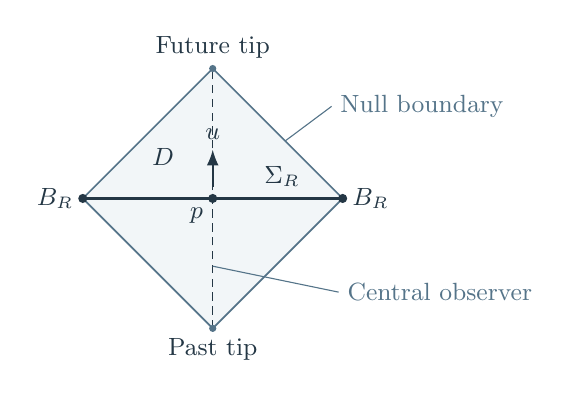
\begin{tikzpicture}[paper diagram]
  \coordinate (past) at (0,-1.65);
  \coordinate (future) at (0,1.65);
  \coordinate (left) at (-1.65,0);
  \coordinate (right) at (1.65,0);

  \fill[diagramfill] (past)--(left)--(future)--(right)--cycle;
  \draw[diagramborder,semithick] (past)--(left)--(future)--(right)--cycle;
  \draw[diagramink,densely dashed] (past)--(future);
  \draw[diagramink,very thick] (left)--(right);
  \draw[paper arrow] (0,.14)--(0,.62) node[above] {$u$};
  \fill[diagramink] (left) circle (1.65pt)
    (right) circle (1.65pt) (0,0) circle (1.65pt);
  \fill[diagramborder] (past) circle (1.3pt) (future) circle (1.3pt);
  \node[above] at (future) {Future tip};
  \node[below] at (past) {Past tip};

  \node[below left] at (0,0) {$p$};
  \node at (-.63,.53) {$D$};
  \node[above] at (.88,.03) {$\Sigma_R$};
  \node[right] at (right) {$B_R$};
  \node[left] at (left) {$B_R$};
  \draw[diagramborder,thin] (.92,.73)--(1.51,1.17)
    node[right,inner xsep=3pt] {Null boundary};
  \draw[diagramborder,thin] (0,-.86)--(1.60,-1.19)
    node[right,inner xsep=3pt] {Central observer};
\end{tikzpicture}
\caption{Schematic radial section of a local causal diamond $D$. The central slice contains the geodesic ball $\Sigma_R$ of radius $R$. The marked ends of its diameter represent the boundary sphere $B_R=\partial\Sigma_R$. The dashed timelike line shows the central observer, with future unit tangent $u$ at the center $p$.}
\label{fig:diamond}
\end{figure}

On the enlarged Hilbert space $\Hh_{\rm QFT}\otimes L^2(\R,\dd q)$ put
\begin{equation}
 H_X=-\log\Delta_{\Omega,\M_X},\qquad p=-i\partial_q,\qquad
 \pi_X(x)=e^{ipH_X}x e^{-ipH_X},\qquad \lambda_X(t)=e^{itq}.
 \label{eq:dressing}
\end{equation}
The energy variable $q$ is dimensionless. Its conjugate $p$ is defined on the full line before imposing positive clock energy. The modular group is $\sigma_t^X(x)=e^{-itH_X}x e^{itH_X}$ and
\begin{equation}
 \lambda_X(t)\pi_X(x)\lambda_X(t)^*=\pi_X(\sigma_t^X(x)).
 \label{eq:covariance}
\end{equation}
The covariance relation follows from $e^{itq}p e^{-itq}=p-t$. In the combined action generated by $H_X+q$, the shift of $p$ cancels the conjugation of $x$ by $e^{itH_X}$, so $\pi_X(x)$ is invariant. This regular representation of the crossed product gives the continuous core
$\Core_X=\M_X\rtimes_{\sigma^X}\R$, represented as the invariant subalgebra of $\M_X\,\bar\otimes\,B(L^2(\R))$ under that action. The positive-energy clock corner is defined by compression with the spectral projection $\Pi=\one_{[0,\infty)}(q)$ after the crossed product has been formed \cite{Takesaki2003,Witten2022,CLPW2022}.

\begin{proposition}[Finite clock corner]
\label{prop:corner}
For $X=D,P$, the algebra $\N_X=\Pi\Core_X\Pi$ is a type-$\mathrm{II}_1$ factor. Its normalized trace is the vector state of
$\Psi_\tau=\Omega\otimes e^{-q/2}\one_{[0,\infty)}(q)$ in the representation \eqref{eq:dressing}.
\end{proposition}

\begin{proof}
The continuous core of a type-$\mathrm{III}_1$ factor is a type-$\mathrm{II}_\infty$ factor by the crossed-product structure theorem \cite{Takesaki2003}. Its canonical semifinite trace is represented by the weight obtained by slicing with $\Omega$ and integrating the clock diagonal against $e^{-q}\dd q$, as in the CLPW trace construction \cite[Sec.~2.4]{CLPW2022}. The sign agrees with the dual action $\theta_s(\lambda_X(t))=e^{-ist}\lambda_X(t)$: it sends $f(q)$ to $f(q-s)$, and the measure $e^{-q}\dd q$ gives the trace scaling factor $e^{-s}$. On positive elements in the domain of the weight, the clock-diagonal formula therefore assigns $\Pi$ the trace $\int_0^\infty e^{-q}\dd q=1$. Restriction to the corner gives the vector formula and a faithful, normal, normalized trace.
\end{proof}

Let $\tau_X$ denote this trace and identify the unit of the corner with $\one$. For a normal state represented by a density $\rho$ relative to $\tau_X$, the entropy with this normalization is
\begin{equation}
 S_{\tau_X}(\rho)=-\tau_X(\rho\log\rho)
                  =-D_{\tau_X}(\rho\Vert\one)\leq0.
 \label{eq:trace-entropy}
\end{equation}
This equality allows the value $-\infty$. The zero sets the entropy of the trace state and fixes the additive normalization. A physical identification of this entropy with $\Sgen$ requires a gravitational model and a specified semiclassical class of states. In particular, the static-patch identification in \cite{CLPW2022} and the general-subregion construction in \cite{Jensen2023} use gravitational constraints to match the algebraic entropy with a geometric area term.

\begin{proposition}[Obstruction to a vacuum-compatible inclusion of cores]
\label{prop:obstruction}
Suppose $\M_D\subsetneq\M_P$ and $\Omega$ is cyclic and separating for both. There is no normal unital embedding $\Core_D\to\Core_P$ that sends $\pi_D(x)$ to $\pi_P(x)$ for every $x\in\M_D$ and sends the clock unitaries $\lambda_D(t)$ to $\lambda_P(t)$ for all $t\in\R$.
\end{proposition}

\begin{proof}
The covariance relation \eqref{eq:covariance}, applied to the proposed images, would imply
$\sigma_t^P(x)=\sigma_t^D(x)$ for $x\in\M_D$. Hence $\M_D$ would be globally invariant under $\sigma^P$. Takesaki's theorem would then give a vacuum-preserving conditional expectation $E:\M_P\to\M_D$ \cite{Takesaki1972}. On vacuum vectors the expectation is implemented by the orthogonal projection $e_D$ onto $\overline{\M_D\Omega}$, so
$E(x)\Omega=e_Dx\Omega$ for $x\in\M_P$. Cyclicity for $\M_D$ implies $e_D=\one$. Since $\Omega$ is separating for $\M_P$, $E(x)=x$ for all $x\in\M_P$. This contradicts proper inclusion.
\end{proof}

The proposition translates the standard Takesaki argument, with vacuum cyclicity of the smaller algebra, to a particular map between the uncompressed cores. Its conclusion concerns the simultaneous identification of the field representation and clock unitaries. Changes of quantum reference frame can involve different observer algebras and additional relational data \cite{DeVuystEtAl2025}. An embedding of the finite corners for such data would require its own construction. Once a unital inclusion between finite factors is specified, a trace-preserving conditional expectation is available.

\section{Standard-form reconstruction in a tracial extension}
\label{sec:code}

The single-diamond corner $\N_D$ serves as the logical algebra. We first state the reconstruction for a general unital inclusion of finite tracial von Neumann algebras and then specify a tracial extension for the model. The left and right actions in the trace GNS representation furnish an algebra and its commutant. Spatial complementary recovery would require a separate identification of the accessible physical algebras.

\begin{proposition}[Tracial inclusion code]
\label{prop:code}
Let $\jmath:(\N,\tau_{\N})\hookrightarrow(\Palg,\tau_{\Palg})$ be a normal unital trace-preserving embedding of finite von Neumann algebras with faithful normalized traces. Define
\begin{equation}
 V:L^2(\N,\tau_{\N})\longrightarrow L^2(\Palg,\tau_{\Palg}),\qquad
 V\widehat{x}=\widehat{\jmath(x)}.
 \label{eq:V}
\end{equation}
Then $V$ is isometric, and left and right logical multiplication are simultaneously reconstructed by left and right multiplication by $\jmath(\N)$ in the physical representation. The compression of a physical left multiplier is the logical left multiplier by $E(y)$, where
$E=\jmath^{-1}\circ E_{\jmath(\N)}$ and $E_{\jmath(\N)}$ is the trace-preserving conditional expectation. For any normal states $\varphi,\psi$ on $\N$,
\begin{equation}
 D_{\Palg}(\varphi\circ E\Vert\psi\circ E)=D_{\N}(\varphi\Vert\psi).
 \label{eq:pres}
\end{equation}
\end{proposition}

\begin{proof}
Trace preservation gives $\|\widehat{\jmath(x)}\|_2=\|\widehat x\|_2$. Multiplicativity gives $L_{\jmath(a)}V=VL_a$ and $R_{\jmath(a)}V=VR_a$, also for adjoints, where $L$ and $R$ denote left and right multiplication. In trace standard form the right multiplication algebra is the commutant of the left algebra. The conditional expectation exists by Takesaki's theorem because the trace has trivial modular flow. For $x,z\in\N$ and $y\in\Palg$,
\[
 \tau_{\Palg}\bigl(\jmath(z)^* y\jmath(x)\bigr)
   =\tau_{\N}\bigl(z^*E(y)x\bigr).
\]
This proves $V^*L_yV=L_{E(y)}$ and the trace-duality relation
$\tau_{\Palg}(\jmath(a)y)=\tau_{\N}(aE(y))$. In particular $\jmath$ is the tracial recovery map for the compression. The same trace duality identifies the physical state density as $\jmath(\rho)$ if the logical state density is $\rho$, with the map extended to trace $L^1$. Monotonicity under $E$ proves one inequality in \eqref{eq:pres}. Applying monotonicity under $\jmath$ and using $E\circ\jmath=\mathrm{id}_{\N}$ proves the other, also with infinite relative entropy \cite{Araki1976,Petz1988}.
\end{proof}

For an explicit diamond code choose
\begin{equation}
 \N=\N_D,\quad \Palg_D=\N_D\,\bar\otimes\,M_2(\C),\quad
 \jmath(x)=x\otimes\one_2,\quad
 E=\mathrm{id}_{\N_D}\,\bar\otimes\,\mathrm{tr}_2,
 \label{eq:example}
\end{equation}
where $\mathrm{tr}_2$ is the normalized matrix trace. Both algebras are type-$\mathrm{II}_1$ factors, and $V\xi=\xi\otimes\widehat{\one_2}$. The code is a noiseless subsystem for discarding the auxiliary matrix factor. All logical information resides in the $\N_D$ factor. The reconstructed right action belongs to the standard-form commutant of the left physical algebra, while the auxiliary factor is a tensor factor of the left algebra. Protection against erasures of logical degrees of freedom would require a different encoding and a specified family of erasures. A geometric realization would also require a map to a physically defined algebra of observables.

Figure~\ref{fig:code} shows the construction of the logical algebra and the two maps for this tracial extension.

\begin{figure}[htbp]
\centering
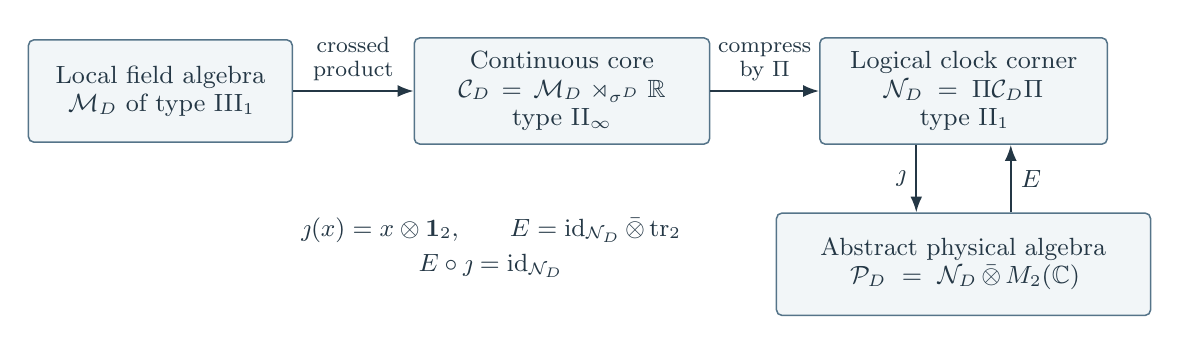
\begin{tikzpicture}[paper diagram]
  \node[paper box,text width=30mm] (field) at (-5.1,0)
    {Local field algebra\\[-.2ex] $\M_D$ of type $\mathrm{III}_1$};
  \node[paper box,text width=34mm] (core) at (0,0)
    {Continuous core\\[-.2ex] $\Core_D=\M_D\rtimes_{\sigma^D}\R$\\[-.2ex]
     type $\mathrm{II}_\infty$};
  \node[paper box,text width=33mm] (logical) at (5.1,0)
    {Logical clock corner\\[-.2ex] $\N_D=\Pi\Core_D\Pi$\\[-.2ex]
     type $\mathrm{II}_1$};

  \draw[paper arrow] (field.east)--(core.west)
    node[midway,above,font=\footnotesize,align=center] {crossed\\[-.2ex] product};
  \draw[paper arrow] (core.east)--(logical.west)
    node[midway,above,font=\footnotesize,align=center] {compress\\[-.2ex] by $\Pi$};

  \node[paper box,text width=44mm] (physical) at (5.1,-2.20)
    {\mbox{Abstract physical algebra}\\[-.2ex] $\Palg_D=\N_D\,\bar\otimes\,M_2(\C)$};
  \draw[paper arrow] ([xshift=-6mm]logical.south)--
    ([xshift=-6mm]physical.north) node[midway,left] {$\jmath$};
  \draw[paper arrow] ([xshift=6mm]physical.north)--
    ([xshift=6mm]logical.south) node[midway,right] {$E$};

  \node[align=center] at (-.90,-1.99)
    {$\jmath(x)=x\otimes\one_2$,\qquad
     $E=\mathrm{id}_{\N_D}\,\bar\otimes\,\mathrm{tr}_2$\\[.45ex]
     $E\circ\jmath=\mathrm{id}_{\N_D}$};
\end{tikzpicture}
\caption{Construction of the finite corner and the tracial inclusion. The map $E$ compresses observables to the logical algebra, and encoding states by precomposition with $E$ preserves relative entropy as in \eqref{eq:pres}. The encoded states share a fixed tracial state on the auxiliary factor.}
\label{fig:code}
\end{figure}

For any inclusion in Proposition~\ref{prop:code}, the normalized physical trace gives the same entropy for $\jmath(\rho)$ as the logical trace gives for $\rho$. This follows from functional calculus with $s\log s=0$ at $s=0$ and trace preservation. An area term in generalized entropy must therefore enter through an independent gravitational identification.

\section{Entropy variation and an exact clock example}
\label{sec:entropy}

Let $\rho_s$ be a differentiable family of state densities in a finite tracial algebra, with faithful reference density $\rho_0$. The operator $K_0=-\log\rho_0$ may be unbounded. Where the entropy and the expectation of $K_0$ are both finite,
\begin{equation}
 D_\tau(\rho_s\Vert\rho_0)
   =-S_\tau(\rho_s)+\tau(\rho_sK_0),\qquad K_0=-\log\rho_0
 \label{eq:first-law}
\end{equation}
If both terms are differentiable at $s=0$, the relative entropy is stationary there by minimality, and $\delta S_\tau=\delta\langle K_0\rangle$. At the trace density $\rho_0=\one$, $K_0=0$. For a general reference density, the modular expectation can vary. The following family makes this explicit even when the clock's differential entropy has zero first variation.

\begin{proposition}[Clock entropy and type-$\mathrm{II}_1$ entropy]
\label{prop:clock}
In the finite corner $\N_D$, fix the QFT vector to $\Omega$. There are smooth, normalized clock probability densities $w_s$ on $[0,\infty)$ for which, at $s=0$,
\begin{equation}
 \delta D_{\tau_D}(\rho_s\Vert\rho_0)=0,\qquad
 \delta\Sobs(w_s)=0,\qquad
 \delta S_{\tau_D}(\rho_s)=-\delta\langle q\rangle_s\ne0.
 \label{eq:counter}
\end{equation}
Here $\rho_s$ is the density of the vector state of $\Omega\otimes\sqrt{w_s}$ and $\Sobs(w)=-\int_0^\infty w\log w\,\dd q$.
\end{proposition}

\begin{proof}
For the Gaussian densities and compactly supported perturbations used below, $e^qw(q)$ is a bounded positive operator in the clock subalgebra. Since $H_D\Omega=0$, the vacuum matrix element of $\pi_D(x)$ on the QFT factor is the scalar multiplication operator $\omega_D(x)\one$. For the corner compression of each Fourier generator $\pi_D(x)\lambda_D(t)$,
\[
 \big\langle\Omega\otimes\sqrt w,\,\Pi\pi_D(x)\lambda_D(t)\Pi
                     \,\Omega\otimes\sqrt w\big\rangle
 =\omega_D(x)\int_0^\infty w(q)e^{itq}\,\dd q .
\]
The trace vector formula gives the same value for
$\tau_D\bigl(e^qw(q)\Pi\pi_D(x)\lambda_D(t)\Pi\bigr)$.
The compressed linear span of these generators is ultraweakly dense. Therefore the exact density is $\rho_w=e^qw(q)$, and
\begin{equation}
 S_{\tau_D}(\rho_w)=\Sobs(w)-\int_0^\infty q w(q)\,\dd q.
 \label{eq:clock-entropy}
\end{equation}

Take $w_0(q)=c_\eps e^{-\eps^2 q^2}$ with $\eps>0$ and $c_\eps$ fixed by normalization. Choose a nonnegative smooth bump $\chi$ supported inside $(0,\infty)$ and positive on an interval. Let $b(q)$ be the residual of $q$ after its orthogonal projection onto $\operatorname{span}\{1,q^2\}$ in $L^2(\chi\dd q)$. Then $h=\chi b$ is smooth and compactly supported, $\int h=\int q^2 h=0$, and $\int qh=\int\chi b^2>0$. The ratio $h/w_0$ is bounded and compactly supported, so $w_s=w_0+sh$ is positive and normalized for sufficiently small $|s|$, and the entropy integrals can be differentiated on that support. The Gaussian tails also give a finite expectation of $K_0(q)=\eps^2 q^2-q-\log c_\eps$. Since $\log w_0$ is affine in $q^2$, $\delta\Sobs=-\int h(1+\log w_0)\,\dd q=0$. Formula~\eqref{eq:clock-entropy} gives the last assertion of \eqref{eq:counter}. The density operators commute in the clock subalgebra, so their relative entropy is $\int_0^\infty w_s\log(w_s/w_0)\,\dd q$. Its derivative is $\int h=0$.
\end{proof}

The example changes the clock at fixed QFT vacuum and uses only the local algebra. It demonstrates that first-order stationarity of relative entropy, even with stationary clock entropy, does not enforce stationarity of $S_{\tau_D}$. If an area variation compensates or constrains a clock variation in a gravitational model, that relation is independent input.

\section{Fixed-volume equilibrium and the linearized equation}
\label{sec:geometry}

This section specializes the small-diamond entanglement-equilibrium argument of Jacobson and Jacobson--Visser to a fixed de Sitter background \cite{Jacobson2016,JacobsonVisser2019}. It specifies the first-order gravitational response that a physical realization of the clock construction would have to reproduce.

Let $g^{(0)}$ be the de Sitter metric and $\Lambda=(d-1)(d-2)/(2\lDS^2)>0$. We take $\Lambda$ to include the renormalized vacuum contribution proportional to $g^{(0)}$ so that $G_{\mu\nu}[g^{(0)}]+\Lambda g^{(0)}_{\mu\nu}=0$. The surviving matter source in what follows is the vacuum-subtracted, renormalized first variation. The background data are a point $p$, a future unit timelike vector $u$ at $p$, a sufficiently small geodesic ball $\Sigma_R$ in the time-symmetric slice normal to $u$, and its edge $B_R$. Write $A$ and $\Vol$ for the area and proper volume and $k$ for the trace of the extrinsic curvature of $B_R$ in $\Sigma_R$ with the outward normal. The conformal Killing field $\xi$ of the diamond is future-directed in the interior and vanishes at $B_R$. Its surface gravity magnitude is $\kappa$, and $n$ is the future unit normal of $\Sigma_R$. Rescaling $\xi$ rescales $\kappa$ by the same positive factor.

We impose the CFT modular-energy condition in the matter sector. In the background diamond the vacuum-subtracted modular expectation obeys
\begin{equation}
 \delta\Smat=\delta\langle K_D^{\rm m}\rangle
 =\frac{2\pi}{\kappa}\int_{\Sigma_R}
          n^\mu\xi^\nu\,\delta\langle T_{\mu\nu}\rangle_{\rm ren}\,\dd\Vol.
 \label{eq:matter-law}
\end{equation}
Here the first equality is the entanglement first law for the state variation on the background. The second uses geometric modular flow and the stress-tensor charge for the conformal symmetry \cite{Brunetti1993,Jacobson2016,JacobsonVisser2019}. The matter input is understood in a scheme in which state-independent vacuum terms are absorbed in the background couplings and any additional boundary contributions are absent or accounted for. A nonconformal theory, or a matter sector with extra state-dependent surface terms, requires a corresponding replacement of \eqref{eq:matter-law}.

We use the Einstein--Hilbert Lagrangian with fixed $\Lambda$ as the geometric input. Denote the linearized metric residual by
$\delta\EE_{\mu\nu}=\delta G_{\mu\nu}+\Lambda\delta g_{\mu\nu}$.
With future $n,\xi$ and $k$ as above, the off-shell causal-diamond identity reads
\begin{equation}
 \frac{\kappa}{8\pi\GN}\bigl(\delta A-k\,\delta\Vol\bigr)
 =-\frac{1}{8\pi\GN}\int_{\Sigma_R}
               n^\mu\xi^\nu\delta\EE_{\mu\nu}\,\dd\Vol .
 \label{eq:diamond}
\end{equation}
The metric variation is evaluated on the background diamond with the embedding of $\Sigma_R$ and the vector field $\xi$ held fixed. In the Iyer--Wald identity, the boundary charge variation in these conventions is $-\kappa\delta A/(8\pi\GN)$. The integral of the symplectic current is $-\kappa k\,\delta\Vol/(8\pi\GN)$, obtained using $\mathcal L_\xi g^{(0)}=2\alpha g^{(0)}$, $\alpha|_{\Sigma_R}=0$ and $n^\mu\nabla_\mu\alpha|_{\Sigma_R}=-\kappa k/(d-2)$. The constraint variation gives the integral of $n^\mu\xi^\nu\delta\EE_{\mu\nu}$ with the sign in \eqref{eq:diamond}. In particular, the normal derivative of the conformal factor contributes even though $\mathcal L_\xi g^{(0)}$ vanishes on the slice \cite{Iyer1994,Bueno2017,JacobsonVisser2019}.

For the purely geometric term, $\delta A-k\,\delta\Vol$ is the fixed-volume area variation. Indeed, sliding the edge of the unperturbed round ball changes its area and volume with ratio $\dd A/\dd\Vol=k$. Compensating the volume variation by such a slide therefore subtracts $k\,\delta\Vol$ from $\delta A$. The matter term in \eqref{eq:matter-law} is vacuum-subtracted on the original background diamond. With these conventions our equilibrium assumption is
\begin{equation}
 \left.\delta\Sgen\right|_{\Vol}
  :=\frac{\delta A-k\,\delta\Vol}{4\GN}+\delta\Smat=0 .
 \label{eq:equilibrium}
\end{equation}
This assumption concerns simultaneous geometric and state variations in the leading Einstein effective description.

The finite clock corner and the tracial code supply neither the area term nor the equilibrium condition in \eqref{eq:equilibrium}. To see the missing step, consider identifying the variations in \eqref{eq:clock-entropy} and \eqref{eq:equilibrium} along an admissible joint variation with stationary clock and matter entropies. In the clock normalization of Section~\ref{sec:corner}, this identification would require
\[
 -\delta\langle q\rangle=\frac{\delta A-k\,\delta\Vol}{4\GN}.
\]
This is a matching condition for such variations. A derivation would have to specify the gravitational constraint and its boundary charge for the diamond. In the static-patch construction of CLPW, the analogous identification uses the horizon-area response to observer energy in a semiclassical regime \cite[Sec.~3.2]{CLPW2022}. For general subregions, Jensen, Sorce and Speranza use gravitational constraints with assumptions on modular flow \cite{Jensen2023}. Here the conditional calculation uses \eqref{eq:equilibrium} directly.

Figure~\ref{fig:equilibrium-logic} summarizes how the variational identities and the equilibrium assumption enter Theorem~\ref{thm:einstein}.

\begin{figure}[htbp]
\centering
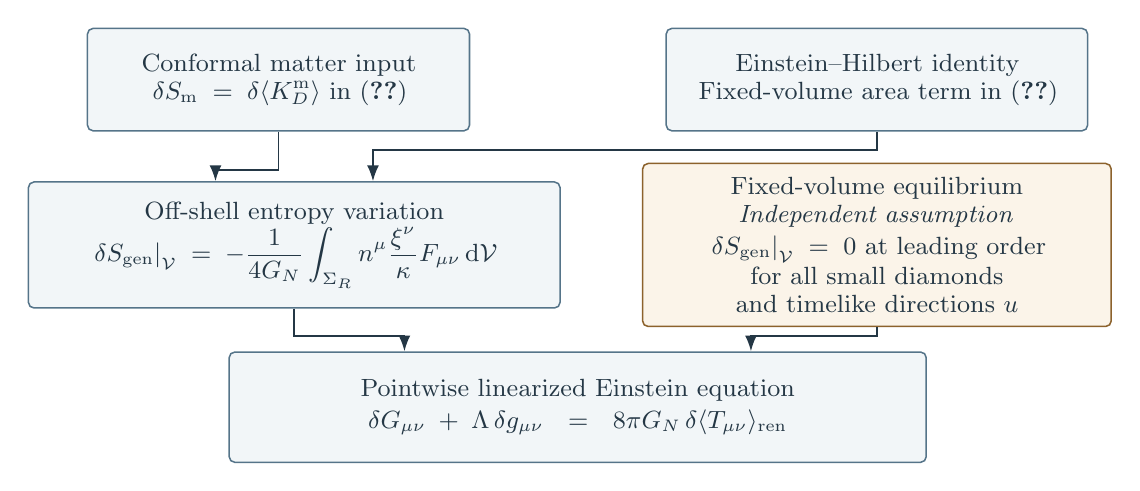
\begin{tikzpicture}[paper diagram]
  \node[paper box,text width=45mm] (matter) at (-3.8,0)
    {Conformal matter input\\[-.2ex]
     $\delta\Smat=\delta\langle K_D^{\rm m}\rangle$ in \eqref{eq:matter-law}};
  \node[paper box,text width=50mm] (gravity) at (3.8,0)
    {Einstein--Hilbert identity\\[-.2ex]
     Fixed-volume area term in \eqref{eq:diamond}};

  \node[paper box,text width=64mm,minimum height=16mm] (identity) at (-3.60,-2.10)
    {Off-shell entropy variation\\[.1ex]
     $\left.\delta\Sgen\right|_{\Vol}=
      -\dfrac{1}{4\GN}\displaystyle\int_{\Sigma_R}
      n^\mu\dfrac{\xi^\nu}{\kappa}F_{\mu\nu}\,\dd\Vol$};
  \node[paper box,draw=diagramwarm,fill=diagrambalance,
        text width=56mm,minimum height=16mm] (assumption) at (3.80,-2.10)
    {Fixed-volume equilibrium\\[-.2ex]
     \emph{Independent assumption}\\[.15ex]
     $\left.\delta\Sgen\right|_{\Vol}=0$ at leading order\\[-.1ex]
     for all small diamonds\\[-.2ex] and timelike directions $u$};

  \draw[paper arrow] (matter.south)--(-3.8,-1.15)-|
    ([xshift=-10mm]identity.north);
  \draw[paper arrow] (gravity.south)--(3.8,-.89)-|
    ([xshift=10mm]identity.north);

  \node[paper box,text width=85mm,minimum height=14mm] (result) at (0,-4.16)
    {Pointwise linearized Einstein equation\\[.15ex]
     $\delta G_{\mu\nu}+\Lambda\,\delta g_{\mu\nu}
      =8\pi\GN\,\delta\langle T_{\mu\nu}\rangle_{\rm ren}$};
  \draw[paper arrow] (identity.south)--(-3.60,-3.26)-|
    ([xshift=-22mm]result.north);
  \draw[paper arrow] (assumption.south)--(3.80,-3.26)-|
    ([xshift=22mm]result.north);
\end{tikzpicture}
\caption{Logical dependencies of the conditional gravitational result. The matter and gravitational identities give the off-shell relation \eqref{eq:integral}, with $F_{\mu\nu}$ the linearized field-equation residual. Imposing fixed-volume equilibrium and extracting the leading small-ball coefficient for every timelike $u$ gives $F_{\mu\nu}=0$ pointwise.}
\label{fig:equilibrium-logic}
\end{figure}

\begin{theorem}[The Jacobson--Visser small-diamond equation on de Sitter]
\label{thm:einstein}
Assume \eqref{eq:matter-law} and the Einstein area term in \eqref{eq:equilibrium}. If \eqref{eq:equilibrium} holds to leading small-ball order for every $p$ and every future unit timelike $u$, then the smooth first variations satisfy
\begin{equation}
 \delta G_{\mu\nu}+\Lambda\,\delta g_{\mu\nu}
      =8\pi\GN\,\delta\langle T_{\mu\nu}\rangle_{\rm ren}.
 \label{eq:einstein}
\end{equation}
Conversely, \eqref{eq:einstein} gives \eqref{eq:equilibrium} at the order where the matter and area variations used above apply.
\end{theorem}

\begin{proof}
Combining \eqref{eq:matter-law} and \eqref{eq:diamond} gives
\begin{equation}
 \left.\delta\Sgen\right|_{\Vol}
 =-\frac{1}{4\GN}\int_{\Sigma_R}
          n^\mu\frac{\xi^\nu}{\kappa}F_{\mu\nu}\,\dd\Vol,\qquad
 F_{\mu\nu}:=\delta\EE_{\mu\nu}
           -8\pi\GN\delta\langle T_{\mu\nu}\rangle_{\rm ren}.
 \label{eq:integral}
\end{equation}
In Riemann normal coordinates centered at $p$, the leading value of $\xi/\kappa$ on the central ball is $(R^2-r^2)u/(2R)$. The proper volume element has Euclidean leading term. Upon rescaling the ball by $R$, smoothness of $F$ and the de Sitter small-ball expansion yield
\begin{equation}
 \int_{\Sigma_R}n^\mu\frac{\xi^\nu}{\kappa}F_{\mu\nu}\,\dd\Vol
   =\frac{\Omega_{d-2}R^d}{d^2-1}\,F_{\mu\nu}(p)u^\mu u^\nu+o(R^d),
 \label{eq:leading}
\end{equation}
where $\Omega_{d-2}$ is the area of the unit $(d-2)$-sphere. The factor in \eqref{eq:leading} follows from
$\Omega_{d-2}\int_0^R r^{d-2}(R^2-r^2)/(2R)\,\dd r$.
Leading-order equilibrium implies $F(u,u)=0$ for every unit future timelike $u$. By homogeneity the quadratic form vanishes on the open timelike cone, hence $F=0$. The converse follows directly from \eqref{eq:integral}.
\end{proof}

The limit in the proof identifies a coefficient in a continuum small-ball expansion. Its effective physical interpretation requires radii large compared with the short-distance cutoff and small compared with $\lDS$ and the variation scales of the sources. This argument takes $\Lambda$ from the chosen comparison geometry. A scalar ambiguity in the entropy variation would add a term proportional to $g^{(0)}_{\mu\nu}$, of the form of a shift $\delta\Lambda\,g^{(0)}_{\mu\nu}$. With a conserved vacuum-subtracted source, the linearized Bianchi identity makes this shift constant. The coefficient of $\delta g_{\mu\nu}$ is the background $\Lambda$ already present in the variational identity \cite{Jacobson2016,JacobsonVisser2019}.

The pointwise metric comparison in Riemann normal coordinates offers a separate geometric observation. If $g$ and $g^{(0)}$ have the same metric and first derivatives at $p$ in a shared chart, then the difference of their Einstein tensors at $p$ is the linearized Einstein tensor of $g-g^{(0)}$ there. The second-derivative part of curvature is linear with coefficients fixed by the common metric at $p$, and the connection-product terms agree. In this chart $\delta g(p)=0$, and the cosmological term at $p$ comes from $G[g^{(0)}](p)=-\Lambda g^{(0)}(p)=-\Lambda g(p)$. Extending Theorem~\ref{thm:einstein} by this observation would require a comparison of states and entropies on the two geometries and an equilibrium statement for the corresponding variations.

\section{Discussion}
\label{sec:limits}

\subsection{Second-order information and horizon questions}

For a twice differentiable density path in the operator norm, with bounded densities and $\rho_0\geq c\one$ for $c>0$, differentiation by the resolvent formula gives
\begin{equation}
 \left.\frac{\dd^2}{\dd s^2}D_\tau(\rho_s\Vert\rho_0)\right|_{s=0}
 =\int_0^\infty\tau\!\left(
    \dot\rho_0(\rho_0+t\one)^{-1}\dot\rho_0(\rho_0+t\one)^{-1}\right)\dd t\geq0 .
 \label{eq:fisher}
\end{equation}
Each integrand is the trace of the square of the self-adjoint operator
$(\rho_0+t\one)^{-1/2}\dot\rho_0(\rho_0+t\one)^{-1/2}$.
Normalization $\tau(\rho_s)=1$ implies $\tau(\ddot\rho_0)=0$, which removes the term linear in $\dd^2\rho_s/\dd s^2$ at the reference. The half-Gaussian reference of Proposition~\ref{prop:clock} has density tending to zero as $q\to\infty$. For that commuting family the second derivative instead follows directly from $\int w_s\log(w_s/w_0)\,\dd q$ and equals $\int h^2/w_0\,\dd q$, finite by compact support. Whenever the Hessian exists, \eqref{eq:pres} gives equality in the logical and physical descriptions for a fixed embedding. A relation to canonical gravitational energy in de Sitter would require a geometric identification of the states, the diamond symplectic data and a corresponding equality of quadratic forms. The holographic AdS calculation provides a comparison under its own assumptions \cite{Hollands2013,LashkariVanRaamsdonk2016,Faulkner2017}.

For an already specified decreasing family of unital finite algebras, restriction of states and of a compatible normalized trace gives monotonicity of $D_\tau(\rho\Vert\one)$ by data processing. A generalized second law would require horizon-cut algebras, a compatible reference state and a geometric entropy identification across cuts. The trace vector gives trivial modular unitaries, and in a proper unital tracial inclusion its orbit under the smaller algebra is confined to a proper subspace. Where the underlying QFT vacuum and the type-$\mathrm{III}$ cut algebras satisfy the Borchers--Wiesbrock hypotheses, their modular inclusion is a separate construction \cite{Borchers1992,Wiesbrock1993}. Lifting it to the finite corners would require compatible embeddings and clock projections across cuts.

The quantum focusing conjecture concerns functional variations with respect to independently movable null generators of a cut \cite{Bousso2016}. Its derivation requires control beyond a single parameter of cut motion, along with the relevant geometry and renormalization. Ceyhan and Faulkner's QFT result supplies a comparison for the quantum null energy condition under specified modular and energy hypotheses \cite{Ceyhan2020}. Chandrasekaran and Flanagan construct horizon-cut algebras with gravitational corner degrees of freedom and analyze generalized entropy and focusing in perturbative gravity \cite{ChandrasekaranFlanagan2026}. Such a construction provides additional physical structure for this question. Likewise, higher-curvature counterterms call for the corresponding entropy functional and generalized volume in the gravitational identity \cite{Bueno2017,Dong2014}. They are independent of corrections to any particular clock wavepacket.

\subsection{Distributed representation and the implicate order}
\label{sec:historical-analogies}

Pribram used optical holography as a model for distributed representation in perception and memory. His holonomic proposal explored Fourier-like transformations in visual processing \cite{Pribram1977}. The analogy with Section~\ref{sec:code} concerns reconstruction across descriptions. For a logical observable $a$, the representative $\jmath(a)$ has expectation $(\varphi\circ E)(\jmath(a))=\varphi(a)$ in the encoded state. In the explicit model \eqref{eq:example}, the representative acts trivially on the auxiliary matrix factor. A correspondence with distributed neural storage would require a separate account of the neural degrees of freedom and the physical implementation of encoding and retrieval.

Bohm used the hologram to illustrate the distinction between an implicate order and the relatively stable forms that unfold from it. He also identified a limit of the analogy. An optical hologram records a pre-existing object, whereas an account of the implicate order must explain how stable forms arise in the first place \cite{Bohm1985}. The same distinction matters for the diamond construction. Its algebra is defined on a specified de Sitter geometry, and the code proves reconstruction for that given region. A stronger emergence claim would require an underlying model that determines which subregions exist and recovers their causal relations. Implementing Bohm's causal interpretation of quantum mechanics would further require specifying the underlying configurations and their guiding dynamics \cite{Bohm1952}.

Gravitational holography poses a dimensional question in addition to these questions of encoding and emergence \cite{Bousso2002}. A horizon interpretation of the code would require identifying its physical algebra with an observable algebra of a lower-dimensional theory and recovering both interior observables and their dynamics. This identification is the step that would give the analogy a geometric realization.

\section{Conclusion}

A finite corner supplies a trace for one diamond. The auxiliary tensor extension illustrates exact standard-form reconstruction and relative-entropy preservation. The modular-flow obstruction constrains a particular choice of embedding into the static-patch core, and the clock example distinguishes stationarity of relative entropy from stationarity of the algebraic entropy. The Jacobson--Visser calculation sets the first-order gravitational response under independent area and fixed-volume equilibrium assumptions. Connecting these results physically would require an embedding into a specified algebra of observables and a constraint on joint variations of state, clock and geometry.

\section{Speculative implications}
\label{sec:implications}

\textbf{The implications in this section are explicitly speculative.} They describe what might follow if the formal results withstand independent scrutiny and, where relevant, their proposed physical interpretation can be established. The suggestions about cosmology, artificial intelligence, and the nature of spacetime have distinct evidential requirements.

\subsection{Scientific implications for quantum gravity}

The reconstruction theorem, the obstruction to a particular modular embedding, and the exact clock example suggest criteria for testing future subregion models. A successful model would specify which observables can be recovered, how the corresponding algebras fit together across overlapping diamonds, and which variations of the observer's energy and of the geometry are jointly allowed. The clock example gives a concrete reason to impose the last criterion. Holding the clock entropy stationary leaves room for changes in the energy that enters the algebraic entropy.

The conditional small-diamond equation identifies the response that such a model would need to reproduce in the conformal matter regime at first order. A stronger result would derive the area contribution and fixed-volume equilibrium from the same microscopic description. In the present calculation the area term and equilibrium enter as assumptions, the variational identity uses the Einstein--Hilbert action, and the positive cosmological constant is set by the comparison geometry. A prediction for cosmology would require additional dynamics and a specified regime in which its observable consequences can be calculated.

\subsection{Relevance to a holographic universe}

A holographic interpretation is motivated by two structures: reconstruction with relative-entropy preservation, illustrated here by a tensor extension, and the area contribution to generalized entropy, which CLPW identifies in an independent semiclassical static-patch model \cite{Bousso2002,CLPW2022}. The construction here uses the bulk diamond algebra itself inside the tensor extension. Giving it a holographic interpretation would require a physically specified lower-dimensional algebra that reproduces interior observables and dynamics and gives compatible descriptions for different observers.

A connection to our universe would further require a realistic cosmological setting in which the proposed identification can be tested. The present results specify properties such a theory should account for. Their realization in a holographic universe remains speculative.

\subsection{Possible implications for AI development}

For classical AI systems, the analogy suggests specifying \emph{which quantities should remain recoverable} and under \emph{which losses of access}. Work on feature superposition in toy neural networks illustrates how a representation can encode features in overlapping directions \cite{Elhage2022}. One could train a model with an extra loss for recovering prespecified task-relevant features after masking groups of activations. Compare standard dropout \cite{SrivastavaEtAl2014}, structured masking with the ordinary task loss, and the same structured masking with the extra feature-recovery loss. Match model size and training budget, and measure both feature recovery and task performance on held-out data and unseen mask patterns. The comparison with structured masking alone isolates the contribution of the extra loss.

In Section~\ref{sec:code}, exact recovery comes from placing all logical information in the unaffected factor. Robustness of learned, distributed representations under activation masking is an empirical question.

\subsection{Philosophical implications}

A construction that recovers geometry and causal relations from an underlying quantum structure would strengthen the case that spacetime can be emergent. A functionalist reading would ask whether that structure can recover the roles through which spacetime is measured, including clock readings, signal propagation, and agreement on local events \cite{LamWuthrich2018}. This gives mathematical content to a question suggested by Bohm's implicate order in Section~\ref{sec:historical-analogies}. How could a more comprehensive description give rise to stable, apparently local structure? The present construction begins with a chosen geometry, so the emergence of that geometry is a further theoretical question.

The observer clock also makes a relational question precise. A clock fixes how observables are defined for a particular observer. De Vuyst and colleagues develop a crossed-product formalism for changing between quantum reference frames, with observer-dependent algebras and entropies \cite{DeVuystEtAl2025}. Recovering a shared spacetime description would additionally require a rule for comparing these observables across overlapping diamonds and recovering the causal relations among them. Even if a bulk description and a lower-dimensional description reproduced the same observations, the question of which description is more fundamental would remain philosophical.

Figure~\ref{fig:speculative-worldview} sketches a possible direction of explanation, from quantum relations to the descriptions available to individual observers. Agreement on shared observables would be a consistency condition for a common spacetime description. Recovering its causal structure and dynamics would require a further derivation.

\begin{figure}[!htbp]
\centering
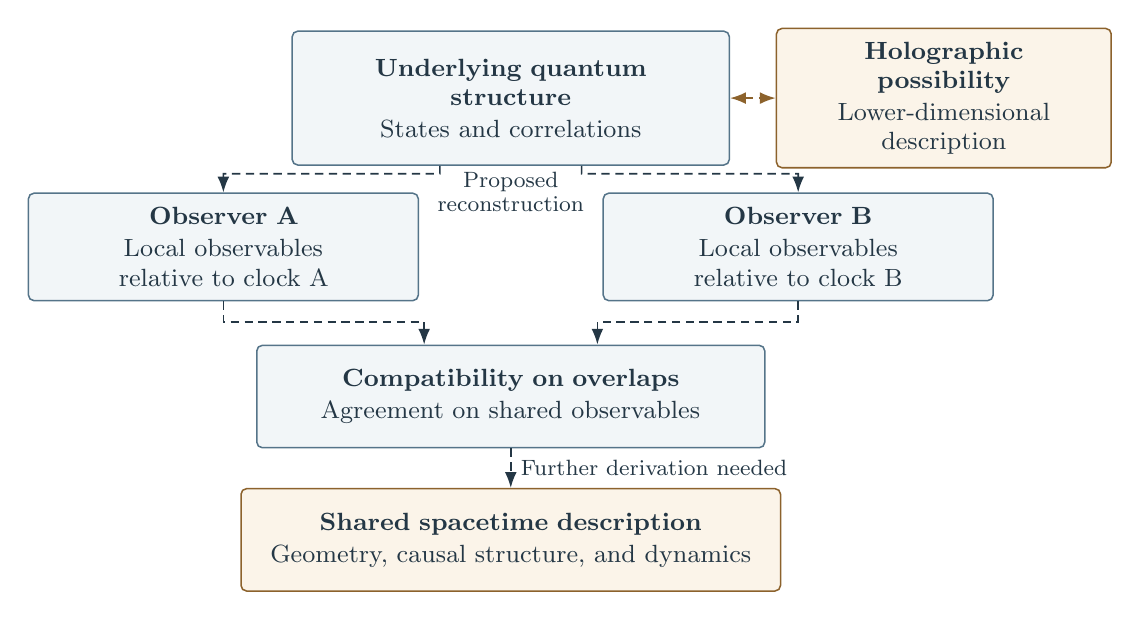
\begin{tikzpicture}[paper diagram,
    conjecture/.style={paper arrow,densely dashed}]
  \node[paper box,text width=52mm,minimum height=17mm] (quantum) at (0,0)
    {\textbf{Underlying quantum}\\[-.16ex] \textbf{structure}\\[.15ex]
     States and correlations};
  \node[paper box,draw=diagramwarm,fill=diagrambalance,text width=39mm,minimum height=17mm]
    (holographic) at (5.5,0)
    {\textbf{Holographic}\\[-.16ex] \textbf{possibility}\\[.15ex]
     Lower-dimensional\\[-.16ex] description};
  \draw[<->,semithick,densely dashed,draw=diagramwarm]
    (quantum.east)--(holographic.west);

  \node[paper box,text width=46mm] (alice) at (-3.65,-1.89)
    {\textbf{Observer A}\\[.15ex]
     Local observables relative to clock A};
  \node[paper box,text width=46mm] (bob) at (3.65,-1.89)
    {\textbf{Observer B}\\[.15ex]
     Local observables relative to clock B};

  \draw[conjecture] ([xshift=-9mm]quantum.south)--(-.9,-.96)-|(alice.north);
  \draw[conjecture] ([xshift=9mm]quantum.south)--(.9,-.96)-|(bob.north);
  \node[font=\footnotesize,align=center] at (0,-1.19)
    {Proposed\\[-.15ex] reconstruction};

  \node[paper box,text width=61mm] (overlap) at (0,-3.79)
    {\textbf{Compatibility on overlaps}\\[.15ex]
     Agreement on shared observables};
  \draw[conjecture] (alice.south)--(-3.65,-2.84)-|([xshift=-11mm]overlap.north);
  \draw[conjecture] (bob.south)--(3.65,-2.84)-|([xshift=11mm]overlap.north);

  \node[paper box,draw=diagramwarm,fill=diagrambalance,text width=65mm]
    (spacetime) at (0,-5.61)
    {\textbf{Shared spacetime description}\\[.15ex]
     Geometry, causal structure, and dynamics};
  \draw[conjecture] (overlap.south)--(spacetime.north)
    node[midway,right,font=\footnotesize] {Further derivation needed};
\end{tikzpicture}
\caption{Speculative worldview for emergent spacetime. Dashed arrows mark proposed links. The holographic possibility is a lower-dimensional description of the underlying quantum structure. The construction in this paper supplies exact reconstruction for one diamond in a specified geometry. The diagram identifies further steps that would be needed to recover a common spacetime.}
\label{fig:speculative-worldview}
\end{figure}

\section*{Acknowledgments}

The original manuscript was prepared with the assistance of Gemini 4 Argon. AI assistance (GPT 6.2 Sol High) was used in the revision.

\begingroup
\small
\let\normalbibliography\thebibliography
\renewcommand{\thebibliography}[1]{%
  \normalbibliography{#1}%
  \setlength{\itemsep}{2pt}%
  \setlength{\parsep}{0pt}%
}
\bibliographystyle{unsrt}
\bibliography{references_de_sitter_oaqec_implications}
\endgroup
\end{document}
